\documentclass[a4paper]{article}


\usepackage{alphabeta} 
\usepackage{enumitem} 
\usepackage{mathtools}
\usepackage{amsmath, amssymb} 
\usepackage{amsthm}
\usepackage{cancel} 
\usepackage[margin=0.70in]{geometry} 
\geometry{left=3cm,right=3cm,top=2.4cm,bottom=2.4cm}	%the page geometry as defined, A4=210x297mm
\usepackage{graphicx}
\usepackage{wrapfig}
\usepackage{caption}
\usepackage{textcomp}
\usepackage{tabto}
\usepackage{layout}
\usepackage{bm}
\usepackage{minipage-marginpar}
\usepackage[dvipsnames]{xcolor}
\usepackage{hyperref}
\usepackage{dutchcal}
\usepackage{derivative}
\usepackage{esint}
%\usepackage{biblatex}
\usepackage{subcaption}
\usepackage{booktabs}\usepackage{derivative}
\usepackage[flushleft]{threeparttable}
\usepackage[capbesideposition=outside,capbesidesep=quad]{floatrow}
\usepackage{derivative}
\usepackage[thinc]{esdiff}
\usepackage{lipsum}
\usepackage{arydshln}
\usepackage[export]{adjustbox}
\usepackage{subcaption}
%%RENEW

\newtheorem{problem}{Άσκηση}
\newtheorem*{solution*}{Λύση}
\newtheorem{definition}{Ορισμός}[subsection]
\newtheorem{properties}{Ιδιότητες}[subsection]
\newtheorem{theorem}{Θεώρημα}[subsection]
\newtheorem{protash}{Πρόταση}[subsection]
\newtheorem{porisma}{Πόρισμα}[subsection]
\newtheorem{lemma}{Λήμμα}[subsection]
\newtheorem*{prooof}{Απόδειξη}
\newtheorem*{notes}{Παρατηρήσεις}
\newtheorem*{note}{Παρατήρηση}
\newtheorem*{app}{Εφαρμογή} 
\newtheorem*{example}{Παράδειγμα}
\newtheorem*{examples}{Παραδείγματα}


\newcommand\numberthis{\addtocounter{equation}{1}\tag{\theequation}}
%\renewcommand{\labelenumi}{\roman{enumi}}
\newcommand{\approxtext}[1]{\ensuremath{\stackrel{\text{#1}}{\approx}}}
\renewcommand{\figurename}{Εικόνα.}
\renewcommand{\tablename}{Πίνακας.}
%\renewcommand\refname{New References Header}
\renewcommand*\contentsname{Περιεχόμενα}
%\DeclareDerivative{\odv}{\mathrm{d}}


\begin{document}
\begin{titlepage}			%makes a title page. Remember to change the author, CID, username and group number to what is appropriate for you!
	\centering
	{\scshape\LARGE Εθνικό Μετσόβιο Πολυτεχνείο\par}
	{\scshape \LARGE Σ.Ε.Μ.Φ.Ε.\par}
	\vspace{1cm}
	{\huge\bfseries Νόμος των Wiedemann-Franz \par}
	\vspace{1cm}
	{\Large\itshape Θωμόπουλος Σπύρος\par}		%remember to change these!
	
	%		{\large Group \@group\unskip\strut\par}
	{\large spyros.thomop@gmail.com/ ge19042@mail.ntua.gr\par \hfill \\}% 		%remember to change these!
	\vspace{1cm}
	{\large Ημερμονηνία Παράδοσης 05/04/2022\par}
\end{titlepage}

\subsection*{Σκοπός}
	
	Ο στόχος της εν λόγω εργαστηριακής άσκησης είναι ο προσδιορισμός της σταθεράς Lorentz (L) χρησιμοποιόντας δύο διαφορετικά μέταλλα, Χαλκό και Νικέλιο.
\subsection*{Θεωρητικά Στοιχεία }

	Κατά τον νόμο Wiedemann-Franz, σε θερμοκρασίες μεγαλύτερες της θερμοκρασίας Debye  ισχύει ότι ο λόγος θερμικής προς ηλεκτρικής αγωγιμότητας των μετάλλων είναι σταθερός και συγκεκριμένα: 
	\begin{align*}\label{1}
		\frac{\lambda}{\sigma } = L T, \hspace{0.7cm} για \hspace{0.2cm} T>T_{Debye} \numberthis 
	\end{align*}
	 όπου λ είναι η σταθερά του Lorentz, η οποία προκύπτει τόσο κλασικά, οσο και κβαντομηχανικά. 
	 
	 \subsubsection*{Κλασικά}
	 	Θεωρούμε πως τα ελεύθερα ηλεκτρόνια ενός μετάλλου απαρτίζουν ένα αέριο και ως αποτέλεσμα της τυχαίας τους κίνησης έχουν μέση ταχύτητα 0 και είναι αυτά που ευθύνονται για τις θερμικές και ηλεκτρικές ιδιότητές του. Αν εφαρμόσουμε ένα ηλεκτρικό πεδίο στο μέταλλο, τότε η κίνηση των ηλεκτρονίων γίνεται κατά την φορά του πεδίου $\vec{E}$ και έτσι έχουμε ηλεκτρικό ρεύμα με 
	 	\begin{align*}\label{2}
	 		\vec{J} =n_0 e \overline{\textbf{u}} \numberthis
	 	\end{align*}
	 Η δύναμη που ασκείται στα ηλεκτρόνια μέσω του πεδίου προκαλλεί μία επιτάχυνση. Ωστόσο η μέση ταχύτητα δεν λαμβάνει αυθαίρετα μεγάλες τιμές καθώς περιορίζεται από τις συγκρούσεις με τα ιόντα του κρυσταλλικού πλέγματος. Εν τέλει προλύπτει ότι 
	 \begin{align*}\label{3}
	 	\vec{J} = n_0e^2\frac{\tau}{2m}\vec{E} \stackrel{\text{Ohm}}{=} \sigma\vec{E} \Rightarrow \\ 
	 	    \sigma = n_0 e^2\frac{\tau}{2m} \numberthis
	 \end{align*}
	 όπου $\tau$ είναι ο μέσος χρόνος μεταξύ των συγκρούσεων των ηλεκτρονίων με τα ιόντα.
	 
	 Αντίστοιχα, η θερμική αγωγιμότητα για την κλασική προσέγγιση είναι 
	 	\begin{align*}\label{4}
	 		\lambda = \frac{n_0 C_e \overline{l}\overline{u}}{3} \numberthis
	 	\end{align*}
	 	όπου $\overline{u}$ η μέση ταχύτητα των e, $\overline{l}$ η μέση ελέυθερη διαδρομή τους και $C_e=3κ/2$ η θερμοχωρητικότητά τους.
	 Έτσι, προκύπτει η σταθερά Lorentz
	 	\begin{align*}\label{5}
	 		L = \frac{8}{\pi} \frac{k^2}{e^2}\simeq 1.9\times10^{-8} W\Omega K^{-2}  \numberthis
	 	\end{align*}
	 \subsubsection*{Κβαντομηχανικά}
	 
	 Ομοίως με πριν, θεωρούμε ότι τα ελεύθερα ηλεκτρόνια απαρτίζουν ένα αέριο αλλά πλέον έχει συμπεριληφθεί η στατιστική Fermi-Dirac και η απαγορευτική αρχή του Pauli που ισχύουν για τα ηλεκτρόνια εφόσον είναι φερμιόνια και οι οποίες έχουν ως συνέπεια την εμφάνιση ενός κατώτατου ορίου για την ενέργεια που μπορεί να έχει ένα ηλεκτρόνιο, την ενέργεια Fermi, $E_f$	. Εδώ το μόνο που αλλάζει είναι οι τιμές των μεγεθών $\overline{u},\overline{l},\tau $ και $ C_e$.
	 
	 Το τελικό αποτέλεσμα της σταθεράς Lorentz προκύπτει κοντα σε αυτό της κλασικής προσέγγισης αλλά είναι πιό κοντά στο αποδεκτό: 
	 	\begin{align}\label{6}
	 		L = \frac{\pi^2}{3}\frac{k^2}{e^2} = 2.45 \times10^{-8} W\Omega K^{-2}
	 	\end{align}

	\subsubsection*{Μέθοδος που χρησιμοποιείται}	
	
	Θα μετρήσουμε τον λόγο $\sigma/\lambda$ με ένα πείραμα.  Κρατάμε την θερμοκρασία της ράβδου στα άκρα της σταθερή, φέρνοντάς την σε επαφή με σώμα μεγάλης θερμοχωρητικότητας και διοχετεύουμε σε αυτήν ρεύμα $I_0$ το οποίο προκαλεί έκλυση θερμότητας εντός της ράβδου με ρυθμό $f(x)$ ανά μονάδα όγκου. Αν θεωρήσουμε ότι δεν εκλύεται θερμότητα από την πλευρική επιφάνεια της ράβδου και επίσης $Q_1$ την θερμότητα που εισέρχεται σε ένα στοιχειώδες κομμάτι της ράβδου (x,x+dx), $Q_2$ την θερμότητα που εκλύεται εντός του όγκου, $Q_3$ την θερμότητα που εξέρχεται και $Q_4$ την θερμότητα που απορροφάται, τότε από την Αρχή Διατήρησης της Ενέργειας έχουμε: 
		\begin{align*}
			Q_1+Q_2=Q_3+Q_4 & \overset{Q_2=f(x)sdxdt, Q_4=C\rho sdx\pdv{T}{t}dt}{\underset{Q_1,Q_3 ν. αγωγης θερμ.}\Rightarrow} \\ 
								&\vdots \\
					\frac{\rho C}{\lambda} \pdv{T}{t} = \pdv[2]{T}{x} +\frac{f}{\lambda} \numberthis
		\end{align*}
		
	Για την μόνιμη κατάσταση έχουμε $\pdv{T}{t}=0$ και θεωρούμε σταθερές τις ιδιότητες της ράβδου καθώς το κέντρο θα είναι θερμότερο μόνο κατά $2^0C$ απ' τα άκρα, άρα 
	\begin{align}
		f=\frac{W}{V}=\frac{I_0^2R}{sl}=\frac{V^2}{Rsl}
	\end{align}
	
		Εν τέλει, έπειτα από 2 ολοκληρώσεις και εφαρμόζοντας την συνθήκη μεγίστου της θερμοκρασίας για το κέντρο της ράβδου, παίρνουμε την λύση 
			\begin{align*}
				T(x) = \frac{f}{2\lambda}	\left(\frac{l^2}{4}-x^2\right) + T_0 \numberthis
			\end{align*}	
			
 	Για $x=0$ παίρνουμε: 
 		\begin{align*}\label{10}
 			V^2 = \frac{8\lambda}{\sigma }\Delta T, \hspace{1cm} \text{για $\Delta T = T(0)-T_0$} \numberthis
		\end{align*} 	
		
		Συνεπώς με μία μέθοδο ελαχίστων τετραγώνων μπορούμε να υπολογίσουμε τον λόγο $\lambda/\sigma$ και κατ' επέκταση της σταθερά Lorentz  
		\begin{align}
			L = \frac{\lambda}{\sigma T}	
		\end{align}					 	
\subsection*{Πειραματική Διάταξη}
	Η διάταξη αποτελείται από: 
		\begin{itemize}
			\item[.] Πηγή ρεύματος $0-20Α$
			\item[.] Σύρμα χαλκού (καλός αγωγός) και νικελίου (κακός αγωγός) με διάμετρο 2mm και μήκος 80mm
			\item[.] Δύο βάσεις μεγάλης θερμοχωτητικότητας όπου στερεώνουμε τις άκρες των συρμάτων 
			\item[.] Ένα θερμόμετρο 
			\item[.] Ένα βολτόμετρο
		\end{itemize}
		Φαίνεται στην Εικόνα (\ref{Im1})
		
		\begin{figure}[h!]
			\centering
			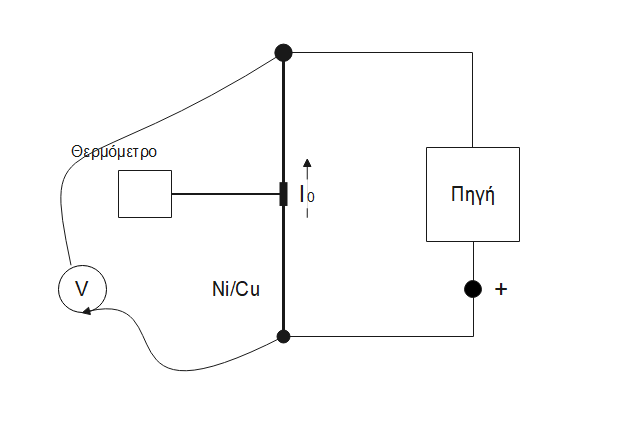
\includegraphics[width=0.45\linewidth]{setup.png}
			\caption{ }
			\label{Im1}
		\end{figure}
		
\subsection*{Πειραματική Διαδικασία - Επεξεργασία Μετρήσεων}
	\subsubsection*{Για το Νi}
		Ανοίγουμε το τροφοδοτικό και αφπύ περιμένουμε προκειμένου να σταθεροποιηθεί, καταγράφουμε την θερμοκρασία στο κέντρο της ράβδου η οποία θα ταυτίζεται με αυτή των άκρων καθώς η ράβδος βρίσκεται σε θερμική ισορροπία, $T_0=15.2^oC$. Αυξάνοντας το ρεύμα παρατηρούμε πτώση τάσης στα άκρα της ράβδου. Έτσι, αυξάνουμε το ρεύμα για τάσεις $v=1-12mV$ και με βήμα $1mV$ και σε κάθε βήμα αφού περιμένουμε λίγο καταγράφουμε την θερμοκρασία στο κέντρο της ράβδου. Τα αποτελέσματα φαίνονται στον Πίνακα (\ref{mat1}) 
		\begin{table}[h!]
			\centering
			\begin{tabular}{r|r|r|r}
				V(mV) & $V^2(\mu V^2)$ & $Τ(0) (\pm0.1^oC)$ & $\Delta T(\pm0.1^oC)=\Delta T(\pm0.1K)$ \\\hline\hline
				0&0&15.2&0\\
				1&1&15.3&0.1\\
				2&4&15.4&0.2\\
				3&9&15.5&0.3\\
				4&16&15.7&0.5\\
				5&25&15.9&0.7\\
				6&36&16.1&0.9\\
				7&49&16.4&1.2\\
				8&64&16.7&1.5\\
				9&81&17.1&1.9\\
				10&100&17.5&2.3\\
				11&121&17.9&2.7\\
				12&144&18.3&3.1
			\end{tabular}
			\caption{ Μετρήσεις για το Ni }
			\label{mat1}
		\end{table}
		
		Αν θέσουμε $Y=V^2$, $X=\Delta T$, τότε μπρούμε να εφαρμόσουμε ελάχιστα τετράγωνα για την σχέση (\ref{10}) έτσι ώστε $Y=AX+B$, όπου η κλίση θα είναι ίση με $A=8\lambda/\sigma$. Πρακούπτουν τα παρακάτω 
		\begin{align*}
			A_{Ni}= 8\left(\frac{\lambda}{\sigma}\right)_{Ni} = (  46.63 \pm 0.73  ) [10^{-6}W\Omega K^{-1} ] \Rightarrow \\
			\left(\frac{\lambda}{\sigma}\right)_{Ni}  = (  5.83 \pm 0.09  ) [10^{-6}W\Omega K^{-1} ] \numberthis
		\end{align*}
		
		Η Γραφική παράσταση φαίνεται στην Εικόνα (\ref{Im2})
		\begin{figure}[h!]
			\centering
			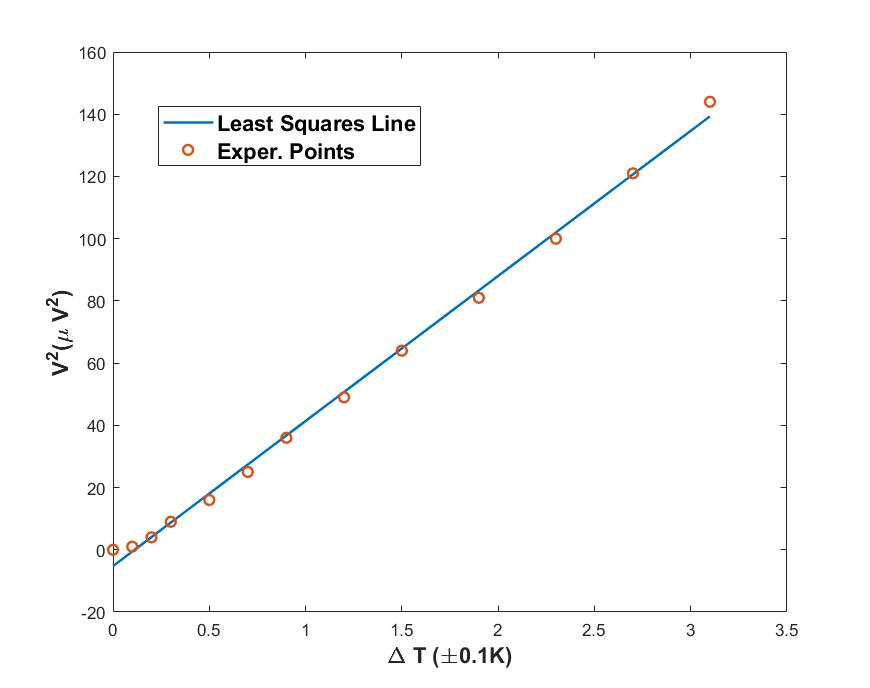
\includegraphics[width=0.7\linewidth]{plot_ni.jpg}
			\caption{ }
			\label{Im2}
		\end{figure}
		
		Για να βρούμε την σταθερά Lorentz πρέπει να διαιρέσουμε την σχέση (12) με την μέση θερμοκρασία της ράβδου. Επειδή η συνολική μεταβολή της κατά την διάρκεια του πειράματος είναι σχετικά μικρή $\sim3^oC$, θα βρω την μέση τιμή της ως εξής
		\begin{align*}
			\overline{T}_{Ni} = \frac{T_{final}+T_0}{2} = 16.8^oC = (16.8+273.2)K \Rightarrow \overline{T}_{Ni} =( 290.0\pm 0.1)K
		\end{align*}
		
		Άρα η σταθερά Lorentz υπολογισμένη από το Ni προκύπτει
	
		\begin{align*}
			L = \left( \frac{1}{\overline{T}_{Ni}}\left(\frac{\lambda}{\sigma}\right)_{Ni} \pm \delta L\right) \Rightarrow 
			  L = ( 2.01\pm0.03 )\times10^{-8}W\Omega K^{-2} \footnotemark  
		\end{align*}
			\footnotetext{Το σφάλμα προκύπτει από διάδοση $\delta L = \sqrt{\left(\pdv{L}{\overline{T}}\delta \overline{T} \right)^2 + \left( \pdv{L}{\lambda/\sigma}\delta (\lambda/\sigma) \right)^2} = \frac{1}{T}\sqrt{ \frac{1}{T^2}(\delta T)^2(\lambda/\sigma)^2 + (\delta(\lambda/\sigma))^2 }$}	
			
			Η διαφορά από την σταθερά που δίνεται στον Πίνακα ($2.14\times10^{-8}W\Omega K^{-2}$) είναι της τάξης του $\sim6\%$. Η απόκλιση αρχικά ίσως οφείλεται στο θεωρητικό μοντέλο που χρησιμοποιήσαμε το οποίο για παράδειγμα δεν περιέχει τις απώλειες θερμότητας από τις πλαϊνές επιφένειες της ράβδου. Ακόμη, ίσως οφείλεται στο γεγονός ότι η θερμοκρασία της ράβδου στα άκρα δεν είναι ακριβώς σταθερή αλλά θα μεταβάλλεται κατά την διάρκειεα του πειράματος. Ίσως να έπρεπε να υπάρχει μεγαλύτερος χρόνος μεταξύ των διαδοχικών μετρήσεων ώστε να υπήρχε ο απαραίτητος χρόνος ώστε να επιτευγχθεί η θερμική ισορροπία της ράβδου.
			
		\subsubsection*{Για τον Cu}
			Εδώ επαναλαμβάνονται ακριβώς τα ίδια βήματα με πριν. Τα αποτελέσματα των μετρήσεων βρίσκονται στον Πίνακα (\ref{mat2}) και η 		γραφική παράσταση που προκύπτει από την μέθοδο των ελαχίστων τετραγώνων φαίνεται στην Εικόνα (\ref{im3}). 
			
			\begin{table}[h!]
				\centering
				\begin{tabular}{r|r|r|r}			
					V(mV) & $V^2(\mu V^2)$ & $Τ(0) (\pm0.1^oC)$ & $\Delta T(\pm0.1^oC)=\Delta T(\pm0.1K)$ \\\hline\hline
					0&0&15.7&0\\
					1&1&15.8&0.1\\
					2&4&15.9&0.2\\
					3&9&16&0.3\\
					4&16&16.2&0.5\\
					5&25&16.4&0.7\\
					6&36&16.7&1.0\\
					7&49&17.1&1.4
				\end{tabular}
				\caption{Μετρήσεις για τον Cu}
				\label{mat2}
			\end{table}
			
			Εδώ προκύπτει ότι  
				\begin{align*}
					A_{Cu} = 8\left(\frac{\lambda}{\sigma}\right)_{Cu} = (36.82 \pm 0.98) [10^{-6}W\Omega K^{-2}] \Rightarrow \\ 
					\left(\frac{\lambda}{\sigma}\right)_{Cu} = ( 4.60 \pm 0.12) [10^{-6}W\Omega K^{-2}]
				\end{align*}
				
				και επίσης $\overline{T}_{Cu} = (289.6 \pm0.1)K$. \\
				
				Άρα η σταθερά Lorentz είναι 	
					
		\begin{align*}
			L = \left( \frac{1}{\overline{T}_{Ni}}\left(\frac{\lambda}{\sigma}\right)_{Ni} \pm \delta L\right) \Rightarrow 
			  L = ( 1.59\pm0.04 )\times10^{-8}W\Omega K^{-2} \footnotemark  
		\end{align*}
			\footnotetext{Το σφάλμα προκύπτει όπως και πριν από διάδοση $\delta L = \sqrt{\left(\pdv{L}{\overline{T}}\delta \overline{T} \right)^2 + \left( \pdv{L}{\lambda/\sigma}\delta (\lambda/\sigma) \right)^2} = \frac{1}{T}\sqrt{ \frac{1}{T^2}(\delta T)^2(\lambda/\sigma)^2 + (\delta(\lambda/\sigma))^2 }$}	
				
				\newpage
				
			\begin{figure}[!h]
				\centering
				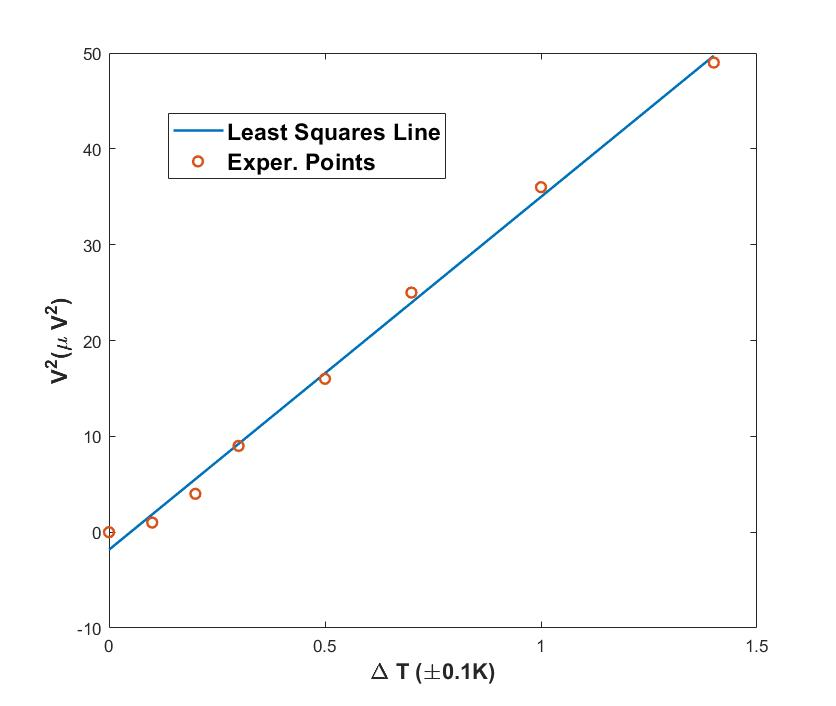
\includegraphics[width=0.7\linewidth]{plot_cu.jpg}
				\caption{ }
				\label{im3}
			\end{figure}
			
			Εδώ παρατηρούμε ότι το σχετικό σφάλμα από την τιμή που δίνεται στον Πίνακα ($2.27\times10^{-8}\Omega K^{-2}$) είναι $\sim30\%$. Η απόκλιση αυτή οφείλεται σε όλους τους λόγους που έχουν αναφερθεί παραπάνω για την απόκλιση του Ni. 
			
			
\subsection*{Συμπεράσματα}


	Τελικά, παρατηρούμε πως εφαρμόζοντας την παραπάνω πειραματική διαδικασία φαίνεται εκ πρώτης όψεως πως το αποτέλεσμα για την σταθερά Lorentz όπως προκύπτει από το Ni, που είναι ο κακός αγωγός, είναι καλύτερο από το αποτελέσμα που δίνει ο Cu, που είναι ο καλός αγωγός, καθώς δίνουν σχετικό σφάλμα $\sim6\%$ και $\sim30\%$ αντίστοιχα από τις αναμενόμενες τιμές. Κάτι τέτοιο πηγαίνει κάπως αντίθετα από την διαίσθησή μας καθώς θα περιμέναμε ότι ο καλός αγωγός θα δίνει καλύτερα αποτελέσματα. 
	
	Παρ' ολ' αυτά ίσως να μην είναι και τόσο σωστό να συγκίρνουμε τα αποτελέσματα που προκύπτουν από τόσο διαφορετικό αριθμό μετρήσεων. Συγκεκριμένα, για το Νικέλιο είχαμε 13 ενώ για τον Χαλκό 8 μετρήσεις, δηλαδή περίπου $40\%$ λιγότερες. Έτσι, μιας και αυτή είναι η μόνη παράμετρος που μπορεί να ελεγχθεί σε αυτό το σημείο, θα υπολογίσω την σταθερά Lorentz μόνο με τις 8 πρώτες μετρήσεις για το Νικέλιο. Με τις ίδιες μεθόδους προκύπτει ίση με $L_{Ni,0-7} = ( 1.83 \pm 0.07 ) \times10^{-8}W\Omega K^{-2}$.  Εδώ, το σχετικό σφάλμα από την αναμενόμενη ($2.14\times10^{-8}W\Omega K^{-2}$) είναι $\sim15\%$. Άρα πράγματι φαίνεται ότι το Νικέλιο να δίνει καλύτερα αποτελέσματα. 
	
	Επομένως, η απόκλιση αυτή από τις αναμενόμενες τιμές οφείλεται σε κάποιο εγγενές χαρακτηριστικό της διάταξης. Ένα από αυτά θα μπορούσε να είναι το γεγονός ότι παρατηρούμε πως τα χάλκινα καλώδια από τα οποία αποτελείται το κύκλωμα έχουν μεγαλύτερη θερμοκρασία στο μέρος που μελετάμε την χάλκινη ράβδο, που σημαίνει ότι έχει αυξηθεί η αντίστασή τους, άρα ίσως επηρεάζονται τα αποτελέσματα.
\end{document}